% Options for packages loaded elsewhere
\PassOptionsToPackage{unicode}{hyperref}
\PassOptionsToPackage{hyphens}{url}
\PassOptionsToPackage{dvipsnames,svgnames,x11names}{xcolor}
%
\documentclass[
  letterpaper,
  DIV=11,
  numbers=noendperiod]{scrartcl}

\usepackage{amsmath,amssymb}
\usepackage{lmodern}
\usepackage{iftex}
\ifPDFTeX
  \usepackage[T1]{fontenc}
  \usepackage[utf8]{inputenc}
  \usepackage{textcomp} % provide euro and other symbols
\else % if luatex or xetex
  \usepackage{unicode-math}
  \defaultfontfeatures{Scale=MatchLowercase}
  \defaultfontfeatures[\rmfamily]{Ligatures=TeX,Scale=1}
\fi
% Use upquote if available, for straight quotes in verbatim environments
\IfFileExists{upquote.sty}{\usepackage{upquote}}{}
\IfFileExists{microtype.sty}{% use microtype if available
  \usepackage[]{microtype}
  \UseMicrotypeSet[protrusion]{basicmath} % disable protrusion for tt fonts
}{}
\makeatletter
\@ifundefined{KOMAClassName}{% if non-KOMA class
  \IfFileExists{parskip.sty}{%
    \usepackage{parskip}
  }{% else
    \setlength{\parindent}{0pt}
    \setlength{\parskip}{6pt plus 2pt minus 1pt}}
}{% if KOMA class
  \KOMAoptions{parskip=half}}
\makeatother
\usepackage{xcolor}
\setlength{\emergencystretch}{3em} % prevent overfull lines
\setcounter{secnumdepth}{5}
% Make \paragraph and \subparagraph free-standing
\ifx\paragraph\undefined\else
  \let\oldparagraph\paragraph
  \renewcommand{\paragraph}[1]{\oldparagraph{#1}\mbox{}}
\fi
\ifx\subparagraph\undefined\else
  \let\oldsubparagraph\subparagraph
  \renewcommand{\subparagraph}[1]{\oldsubparagraph{#1}\mbox{}}
\fi


\providecommand{\tightlist}{%
  \setlength{\itemsep}{0pt}\setlength{\parskip}{0pt}}\usepackage{longtable,booktabs,array}
\usepackage{calc} % for calculating minipage widths
% Correct order of tables after \paragraph or \subparagraph
\usepackage{etoolbox}
\makeatletter
\patchcmd\longtable{\par}{\if@noskipsec\mbox{}\fi\par}{}{}
\makeatother
% Allow footnotes in longtable head/foot
\IfFileExists{footnotehyper.sty}{\usepackage{footnotehyper}}{\usepackage{footnote}}
\makesavenoteenv{longtable}
\usepackage{graphicx}
\makeatletter
\def\maxwidth{\ifdim\Gin@nat@width>\linewidth\linewidth\else\Gin@nat@width\fi}
\def\maxheight{\ifdim\Gin@nat@height>\textheight\textheight\else\Gin@nat@height\fi}
\makeatother
% Scale images if necessary, so that they will not overflow the page
% margins by default, and it is still possible to overwrite the defaults
% using explicit options in \includegraphics[width, height, ...]{}
\setkeys{Gin}{width=\maxwidth,height=\maxheight,keepaspectratio}
% Set default figure placement to htbp
\makeatletter
\def\fps@figure{htbp}
\makeatother
\newlength{\cslhangindent}
\setlength{\cslhangindent}{1.5em}
\newlength{\csllabelwidth}
\setlength{\csllabelwidth}{3em}
\newlength{\cslentryspacingunit} % times entry-spacing
\setlength{\cslentryspacingunit}{\parskip}
\newenvironment{CSLReferences}[2] % #1 hanging-ident, #2 entry spacing
 {% don't indent paragraphs
  \setlength{\parindent}{0pt}
  % turn on hanging indent if param 1 is 1
  \ifodd #1
  \let\oldpar\par
  \def\par{\hangindent=\cslhangindent\oldpar}
  \fi
  % set entry spacing
  \setlength{\parskip}{#2\cslentryspacingunit}
 }%
 {}
\usepackage{calc}
\newcommand{\CSLBlock}[1]{#1\hfill\break}
\newcommand{\CSLLeftMargin}[1]{\parbox[t]{\csllabelwidth}{#1}}
\newcommand{\CSLRightInline}[1]{\parbox[t]{\linewidth - \csllabelwidth}{#1}\break}
\newcommand{\CSLIndent}[1]{\hspace{\cslhangindent}#1}

\KOMAoption{captions}{tableheading}
\makeatletter
\makeatother
\makeatletter
\makeatother
\makeatletter
\@ifpackageloaded{caption}{}{\usepackage{caption}}
\AtBeginDocument{%
\ifdefined\contentsname
  \renewcommand*\contentsname{Table of contents}
\else
  \newcommand\contentsname{Table of contents}
\fi
\ifdefined\listfigurename
  \renewcommand*\listfigurename{List of Figures}
\else
  \newcommand\listfigurename{List of Figures}
\fi
\ifdefined\listtablename
  \renewcommand*\listtablename{List of Tables}
\else
  \newcommand\listtablename{List of Tables}
\fi
\ifdefined\figurename
  \renewcommand*\figurename{Figure}
\else
  \newcommand\figurename{Figure}
\fi
\ifdefined\tablename
  \renewcommand*\tablename{Table}
\else
  \newcommand\tablename{Table}
\fi
}
\@ifpackageloaded{float}{}{\usepackage{float}}
\floatstyle{ruled}
\@ifundefined{c@chapter}{\newfloat{codelisting}{h}{lop}}{\newfloat{codelisting}{h}{lop}[chapter]}
\floatname{codelisting}{Listing}
\newcommand*\listoflistings{\listof{codelisting}{List of Listings}}
\makeatother
\makeatletter
\@ifpackageloaded{caption}{}{\usepackage{caption}}
\@ifpackageloaded{subcaption}{}{\usepackage{subcaption}}
\makeatother
\makeatletter
\@ifpackageloaded{tcolorbox}{}{\usepackage[many]{tcolorbox}}
\makeatother
\makeatletter
\@ifundefined{shadecolor}{\definecolor{shadecolor}{rgb}{.97, .97, .97}}
\makeatother
\makeatletter
\makeatother
\ifLuaTeX
  \usepackage{selnolig}  % disable illegal ligatures
\fi
\IfFileExists{bookmark.sty}{\usepackage{bookmark}}{\usepackage{hyperref}}
\IfFileExists{xurl.sty}{\usepackage{xurl}}{} % add URL line breaks if available
\urlstyle{same} % disable monospaced font for URLs
\hypersetup{
  pdftitle={On the Chicken \& Egg Problem in Transportation Electrification},
  pdfauthor={Jason Hawkins},
  colorlinks=true,
  linkcolor={blue},
  filecolor={Maroon},
  citecolor={Blue},
  urlcolor={Blue},
  pdfcreator={LaTeX via pandoc}}

\title{On the Chicken \& Egg Problem in Transportation Electrification}
\author{Jason Hawkins}
\date{}

\begin{document}
\maketitle
\ifdefined\Shaded\renewenvironment{Shaded}{\begin{tcolorbox}[interior hidden, sharp corners, borderline west={3pt}{0pt}{shadecolor}, breakable, enhanced, boxrule=0pt, frame hidden]}{\end{tcolorbox}}\fi

\hypertarget{introduction}{%
\section{INTRODUCTION}\label{introduction}}

Vehicle electrification is widely regarded as a critical tool for
climate change mitigation in the transportation sector (Musti and
Kockelman 2011). While the United States is seeing an increasing share
of electric sales, the pace of adoption remains well below the necessary
level to mitigate climate change impacts. One barrier to widespread
adoption is the lack of charging infrastructure (Sullivan and Taylor
2021).

A common policy put forward to increase electric vehicle adoption is a
federal income tax credit for EV buyers. However, spending similar
amounts on increasing deployment of charging stations could yield more
effective results (\textbf{Li2017?}). This is especially the case in the
early stages of EV market penetration; EV markets that have
critical-mass constraints have the most success in increasing market
penetration with a subsidy policy that deals with indirect network
effects (\textbf{Zhou2018?}). One of the indirect network effects on the
EV market comes from the charging station market.

Subsidies for charging stations are found to be most effective because
of the low-price sensitivity of early EV adopters (\textbf{Li2017?}).
This is intuitive because early EV adopters are more eager to purchases
EVs, which makes them more willing to pay for higher prices. The issue
these consumers are concerned with is their ability to utilize this new
technology, which is affected by the existing charging station
infrastructure. Because of this, understanding consumer's preferences
for charging station infrastructure is crucial. Consumers are willing to
pay about 5 cents per mile for plug-in electric vehicles and about 10
cents per minute of wait time while refueling. Consumers are also
willing to wait up to 8 minutes longer during refueling
(\textbf{Sheldon2019?}). Knowing this information can allow policy
makers to create subsidy programs that produce more effective outcomes.

Nick TO DO: - Expand discussion to focus on the need for EVs in climate
policy in general (can draw from Net Zero America and Zero Carbon
America studies and others) - Focus on what drives EV adoption according
to literature - Talk about the infrastructure bill and its investment in
charging stations

\begin{verbatim}
C:\Users\jhawkins17\Anaconda3\envs\geo_env\lib\site-packages\seaborn\rcmod.py:400: DeprecationWarning: distutils Version classes are deprecated. Use packaging.version instead.
  if LooseVersion(mpl.__version__) >= "3.0":
C:\Users\jhawkins17\Anaconda3\envs\geo_env\lib\site-packages\setuptools\_distutils\version.py:346: DeprecationWarning: distutils Version classes are deprecated. Use packaging.version instead.
  other = LooseVersion(other)
\end{verbatim}

\hypertarget{the-electric-vehicle-and-charging-station-problem}{%
\section{THE ELECTRIC VEHICLE AND CHARGING STATION
PROBLEM}\label{the-electric-vehicle-and-charging-station-problem}}

Nick TO DO: - More of a technical focus on what's been done in the
academic literature on the specific problem

Electric vehicle ownership is often referenced as exhibiting a ``chicken
and egg'' behavior arising from the supply and demand relationship.
Individual demand for electric vehicles is influenced by the available
supply of charging points. Consumers are unwilling to purchase vehicles
due to range anxiety and a perceived lack of charging stations.
Suppliers are not incentivized to provide charging stations unless there
is sufficient demand to warrant their cost. There is a clear role for
public policy in such situations. The government deems electric vehicles
as a solution to a public ill (i.e., climate change) and can incentivize
either suppliers by providing installation subsidies or consumers by
installing charging stations. While the problem has been recognized in
the literature (Melliger, Vliet, and Liimatainen 2018), empirical
analysis is minimal.

An important consideration to the analysis is how electric mobility
system may differ from one based on fossil fuels. In the conventional
private mobility model, the individual owns the vehicle and purchases
fuel from centralized and privately owned refueling stations. In
contrast, electric vehicles may be charged in the home using previously
existing infrastructure. The presence of charging points in the home
begs the questions 1) if (or to what extent) out-of-home charging
stations are required for travel? and 2) to what extent is range anxiety
a perception versus a reality?

According to the Bureau of Transportation Statistics, 98\% of trips made
in the US are less than 50 miles (Vehicle Technology Office 2022). Given
that most battery-electric vehicles (BEVs) have a range greater than 200
miles (Elfalan 2021), it is feasible to make most trips on a single
charge. However, long-distance trips (over 50 miles) comprise 30\% of
total vehicle-miles traveled (VMT) (Aultman-Hall 2018). There is clearly
a need for out-of-home charging stations to accommodate these trips.
Even if most trips can be accommodated by in-home charging, the vehicle
purchase decision will be influenced by consideration of these longer
trips that require charging stations (Silvia and Krause 2016).
Additionally, Wolbertus et al. (Wolbertus et al. 2018) find that there
is still a demand for charging stations in places where public daytime
charging is the only option, such as at the workplace.

\hypertarget{methods}{%
\section{METHODS}\label{methods}}

We define two classes of causality which we termed as phasing causality
and potential outcomes causality. These alternative forms of causality
are often denoted by their principle developers: Granger causality (REF)
and Rubin causality (REF), respectively. Both approaches are employed
due to the (functionally) continuous nature of the two variables of
interest. We detail each approach and its application to the present
problem below.

\hypertarget{non-linear-phasing-causality}{%
\subsection{Non-Linear Phasing
Causality}\label{non-linear-phasing-causality}}

Define two variables \(X_t\) and \(Y_t\) where subscript \(t\) denotes a
time series process. Phasing causality seeks to identify whether the two
time series exhibit a common pattern (or coherence). One variable may
lead the other producing a time lag, but the series may also exhibit
instantaneous \emph{causality} whereby the current value of \(Y_t\) is
better predicted when the current value of \(X_t\) is included in the
model. In strict terms, phasing causality is defined by
\[\sigma^2(Y|U)<\sigma(Y|\overline{U-X})\] \#\{eq:granger-causality\}.
There is also the potential for feedback, whereby \(X_t\) causes \(Y_t\)
and \(Y_t\) also causes \(X_t\). In the EV and charging station
situation, this might mean that charging station installations encourage
households in a county to purchase EVs, which then encourages further
investment in charging station infrastructure. There are two key
principles underling phasing causality: 1) that the cause occurs before
its effect and 2) that the cause has unique information about the future
values of its effect. Granger defines a simple test statistic for such
causality using time series data using the F-test.

The original applications of Granger causality were to economic
variables that fluctuated over time. The test assumes that both \(X_t\)
and \(Y_t\) are stationary time series, an assumption that will be shown
to be violated in the present case. Several extensions have been
developed to phasing causality that allow for non-stationary time
series. We use the approach of Rosol et al (REF) with modifications to
fit our application as detailed in the following section. Their approach
compares the model median absolute error using both time series (\(Y_t\)
and \$X\_t\$)to that obtained using only the dependent time series
(\$Y\_t\$). The Wilcoxon signed-rank test is used to test for
statistical significance - i.e., that \(X_t\) causes \(Y_t\). The method
is implemented as a Python package and includes multilayer perceptron
(MLP), long short-term memory (LSTM), gated recurrent unit (GRU), and
autoregressive integrated moving average (ARIMA) models. Model errors
are calculated at each observation and the sum of their absolute values
used in the statistical test. The method has the ability to measure
changes in causality over time, but our time series is too short for its
application.

\hypertarget{potential-outcomes-causality-via-propensity-score-matching}{%
\subsection{Potential Outcomes Causality Via Propensity Score
Matching}\label{potential-outcomes-causality-via-propensity-score-matching}}

Potential outcomes causality begins from the definition that causal
effects are a comparison between outcomes \(Y\) in response to
differences in a treatment \(T\) on a common set of units.
Unfortunately, such an analysis is not possible in reality since it
would require the same unit (e.g., person) to simultaneously experience
both the treated and untreated conditions. In observational studies, a
common approach is to identify two sets of observational units that
differ only in their exposure to a treatment variable of interest. A
study interested in the effect of a new teaching strategy might compare
two sets of schools that differ only in whether they adopted the
strategy. A class of strategies to identify otherwise similar
observational units (e.g., schools) is propensity score matching.
Formally, the assumption is that \(Y_t \perp T|X_t\), or that outcome
\(Y_t\) is independent of the treatment conditional upon a set of
\(X_t\) covariates. That is, treatment assignment is ignorable
conditional on \(X_t\). However, for the present problem the treatment
(i.e., charging stations) is not binary. An observation unit may have
any number of charging stations.

An extension to the standard propensity score, termed as generalized
propensity score (GPS) matching, was developed by Hirano and Imbens
(REF). Assuming a continuous treatment, the GPS is defined by
\[r(t,x)=f_{T|X}(t|x)\] \{eq-gps\} where \(t\in \tau\) is referred to as
the unit-level dose-response function, \(X\) and \(T\) are random
variables defined on a common probability space, and \(r(t,x)\) is the
GPS measure defining similarity between observational units. It can then
be stated that \(X\perp 1{T=t}|r(t,X)\), or that assignment to a
treatment value \(t\) is independent conditional on its GPS.

The dose-response nomenclature is taken from pharmeutical research,
where the interest is in the health response to a continuous drug dose.
Each individual has a potential response at different doses, or
treatment levels. The dose-response function that is an outcome of
continuous GPS analysis is an average of the potential responses at each
treatment level - an average dose-response function (ADRF). A challenge
when transitioning from a binary to a continuous treatment is that a
treated unit will not be available at every treatment level. The problem
can be addressed by parameterizing the curve as a linear combination of
a finite number of basis functions (REF Galagate). The averaging used to
construct the ADRF is based on weighting observations by the GPS using
units within each basis function range.

A secondary question is the potential influence of charging stations on
other variables of interest.

\begin{figure}[H]

{\centering 
\includegraphics[width=1.96in,height=0.89in]{TRB_2023_files/figure-latex/mermaid-figure-1.png}

}

\end{figure}

\hypertarget{data-and-model-specification}{%
\section{DATA AND MODEL
SPECIFICATION}\label{data-and-model-specification}}

\hypertarget{treatment-and-outcome-variables}{%
\subsection{Treatment and Outcome
Variables}\label{treatment-and-outcome-variables}}

The two key input datasets are charging station locations provided by
the Alternative Fuel Data Center (AFDC) and electric vehicle
registrations provided by Experian Inc.~The vehicle registration dataset
comprises a 10-year panel at 2-year intervals (2012, 2014, 2016, 2018,
2020). Total vehicle registrations are recorded by county, make, model,
year, and other vehicle characteristics for the United States. The
frequency and spatial resolution of the vehicle registration data define
the analysis units. Our treatment and outcome variables are charging
stations and EV registrations normalized by population (per 100,000
inhabitants).

Charging stations are geocoded and aggregated into annual cumulative
totals by county. Only public charging stations are maintained for
analysis. Further, the we make no distinction between charger port
capacity (level 1, 2, or 3) when aggregating the number of charging
ports per county. Such a distinction could be made as a sensitivity test
but may reduce the effective sample size as not all counties with
charging stations have all three charger port types.

After filtering out protectorates and other non-state locations, several
county codes in the Experian data remain that are missing registration
totals in a subset of years (117/3275, or about 4\%). We remove county
codes with more than one missing year, leaving 34 counties for which
registration totals are interpolated from adjacent years. Many of these
county codes are for remote areas with low populations (e.g., the
Aleutian Islands in Alaska). Of the 3140 viable counties, it is found
that 1406 lack EV registrations or public charging stations in any
analysis year. These counties are excluded from analysis because they
lack variation for model estimation. Figure \textbf{?@fig-missing}
illustrates that a further 80\% of the remaining counties did not have
EV registrations in 2012. While kept in the dataset for analysis, the
high proportion of zero-valued observations poses a significant
challenge for statistical inference.

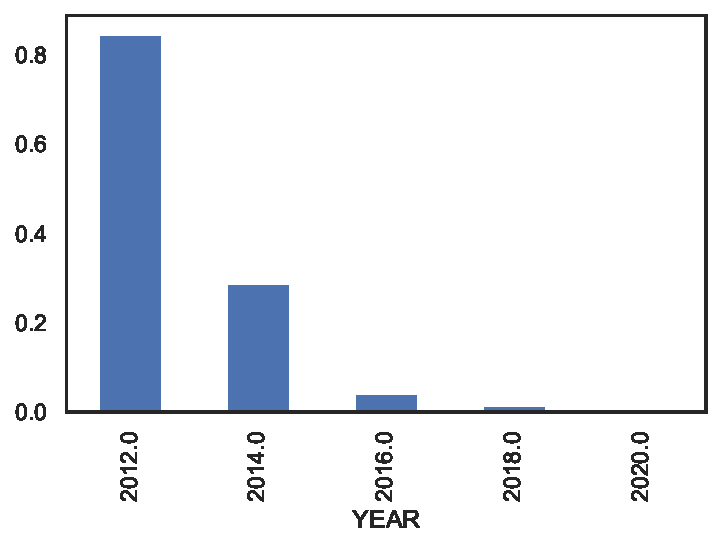
\includegraphics{TRB_2023_files/figure-pdf/cell-9-output-1.pdf}

\hypertarget{covariates}{%
\subsection{Covariates}\label{covariates}}

Census data was compiled to construct county-level statistics for median
income and racial composition. Five-year American Community Survey (ACS)
data were used to approximate annual variation. We use the 2011-2015 ACS
for years 2012 and 2014 and the 2016-2020 ACS for years 2016, 2018, and
2020. For the purposes of analysis, we define minority racial groups as
Black and Hispanic based on an overrepresentation of poverty according
to Census Bureau analysis
(https://www.census.gov/library/stories/2020/09/poverty-rates-for-blacks-and-hispanics-reached-historic-lows-in-2019.html\#:\textasciitilde:text=In\%202019\%2C\%20the\%20share\%20of,share\%20in\%20the\%20general\%20population.).
We also include American Indian and Alaska native, and Native Hawaiian
and Other Pacific Island, and Other Race Not Specified in our
definition.

To capture spatial spillover effects, a Queen contiguity matrix is
constructed for charging station density (per 100,000 inhabitants) in
adjacent counties. The rationale is that an individual may purchase an
EV if there are charging stations in adjacent counties and charge at
their residence when driving in their home county.

Nick TO DO: - Could help describe the data we used a bit

\hypertarget{model-specification}{%
\subsection{Model Specification}\label{model-specification}}

We use the causal-curve Python package developed by Kobrosly (REF). This
package uses a generalized linear model (GLM) to construct the GPS and a
generalized additive model (GAM). The GAM model takes as inputs the GPS,
a treatment grid, and a number of splines. We use the default 100 unit
grid and 30 splines (i.e., separating the GPS space using 30 basis
functions).

\hypertarget{results}{%
\section{Results}\label{results}}

\hypertarget{descriptive-analysis}{%
\subsection{Descriptive Analysis}\label{descriptive-analysis}}

Figure @fig-us-totals provides a first validation of the research
hypothesis. Registered plugin electric vehicles (PEVs) and public
charging stations are normalized by population and plotted over the
eight year analysis period for the United States. The two infrastructure
show a similar exponential increase, suggesting there is a correlation
between their adoption but giving no indication of temporal phasing or
causality.

The classical Granger causality test assumes stationary data, which is
not the case here based on visual inspection and confirmed by ADF and
KPSS tests. Several non-linear extensions to Granger causality have been
developed in recent years (REF). One challenge applying such methods to
our application is that non-linear methods require a larger time series
than the five annual totals purchased from Experian. We address this
limitation by leveraging the multiple observations available in each
year.

Seems unlikely that interaction is occuring at a sub-annual basis given
the time lag and information acquisition requirements between vehicle
purchase and infrastructure construction. Granger: ``Whether or not a
model involving some group of economic variables can be a simple causal
model depends on what one considers to be the speed with which
information flows through the economy and also on the sampling period of
the data used. It might be true that when quarterly data are used, for
example, a simple causal model is not sufficient to explain the
relationships between the variables, while for monthly data a simple
causal model would be all that is required. Thus, some nonsimple causal
models may be constructed not because of the basic pro- perties of the
economy being studied but because of the data being used.''

\begin{figure}

\begin{minipage}[t]{\linewidth}

{\centering 

\raisebox{-\height}{

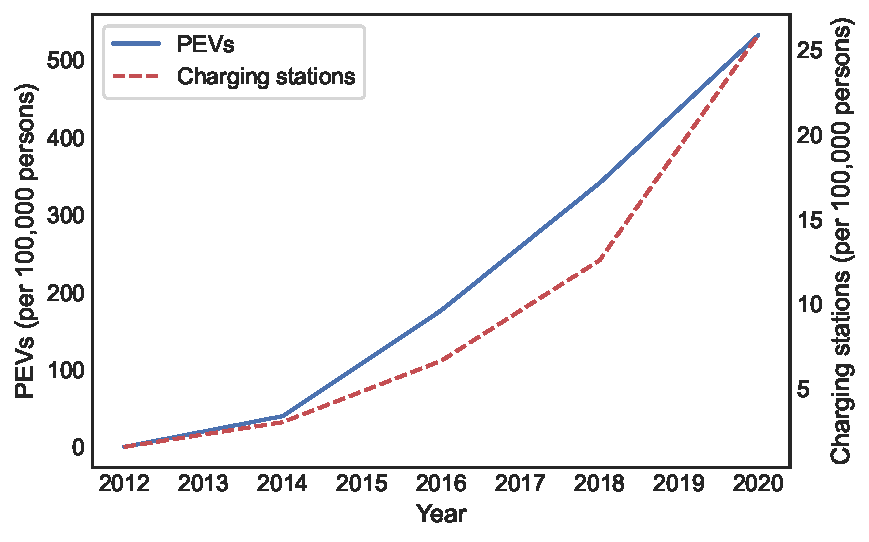
\includegraphics{TRB_2023_files/figure-pdf/fig-us-totals-output-1.pdf}

}

\caption{\label{fig-us-totals}US BEV Registrations and Charging
Stations}

}

\end{minipage}%

\end{figure}

The Bipartisan Infrsatructure Act places a strong focus on equitable
investment allocation. Equity can be explored both inter-regionally and
intra-regionally by key demographic features. Figure 2 compares the
distribution of charging stations for four representative cities. Omaha
is located in the central Great Plains, a region that has received
minimal exploration in the EV literature. Chicago and Detroit are large
cities with well-documented histories of housing segregation (REF). San
Francisco is included as an example of a large city in a progressive
state. In all four cities, charging stations are concentrated in the
central city. San Francisco does not show clear evidence of inequality,
likely partially as a function of the overall high density of charging
stations. However, Chicago and Detroit both show clear patterns of low
charging station density in their majority-minority communities and
unexpectedly high station densities in low density suburban communities.
While there are few charging stations in Omamah, those outside its
downtown are located along an east-west axis along the I-80 corridor.
There are few stations in north and south Omaha, which are enclaves of
black and hispanic residents, respectively.

\begin{figure}

{\centering 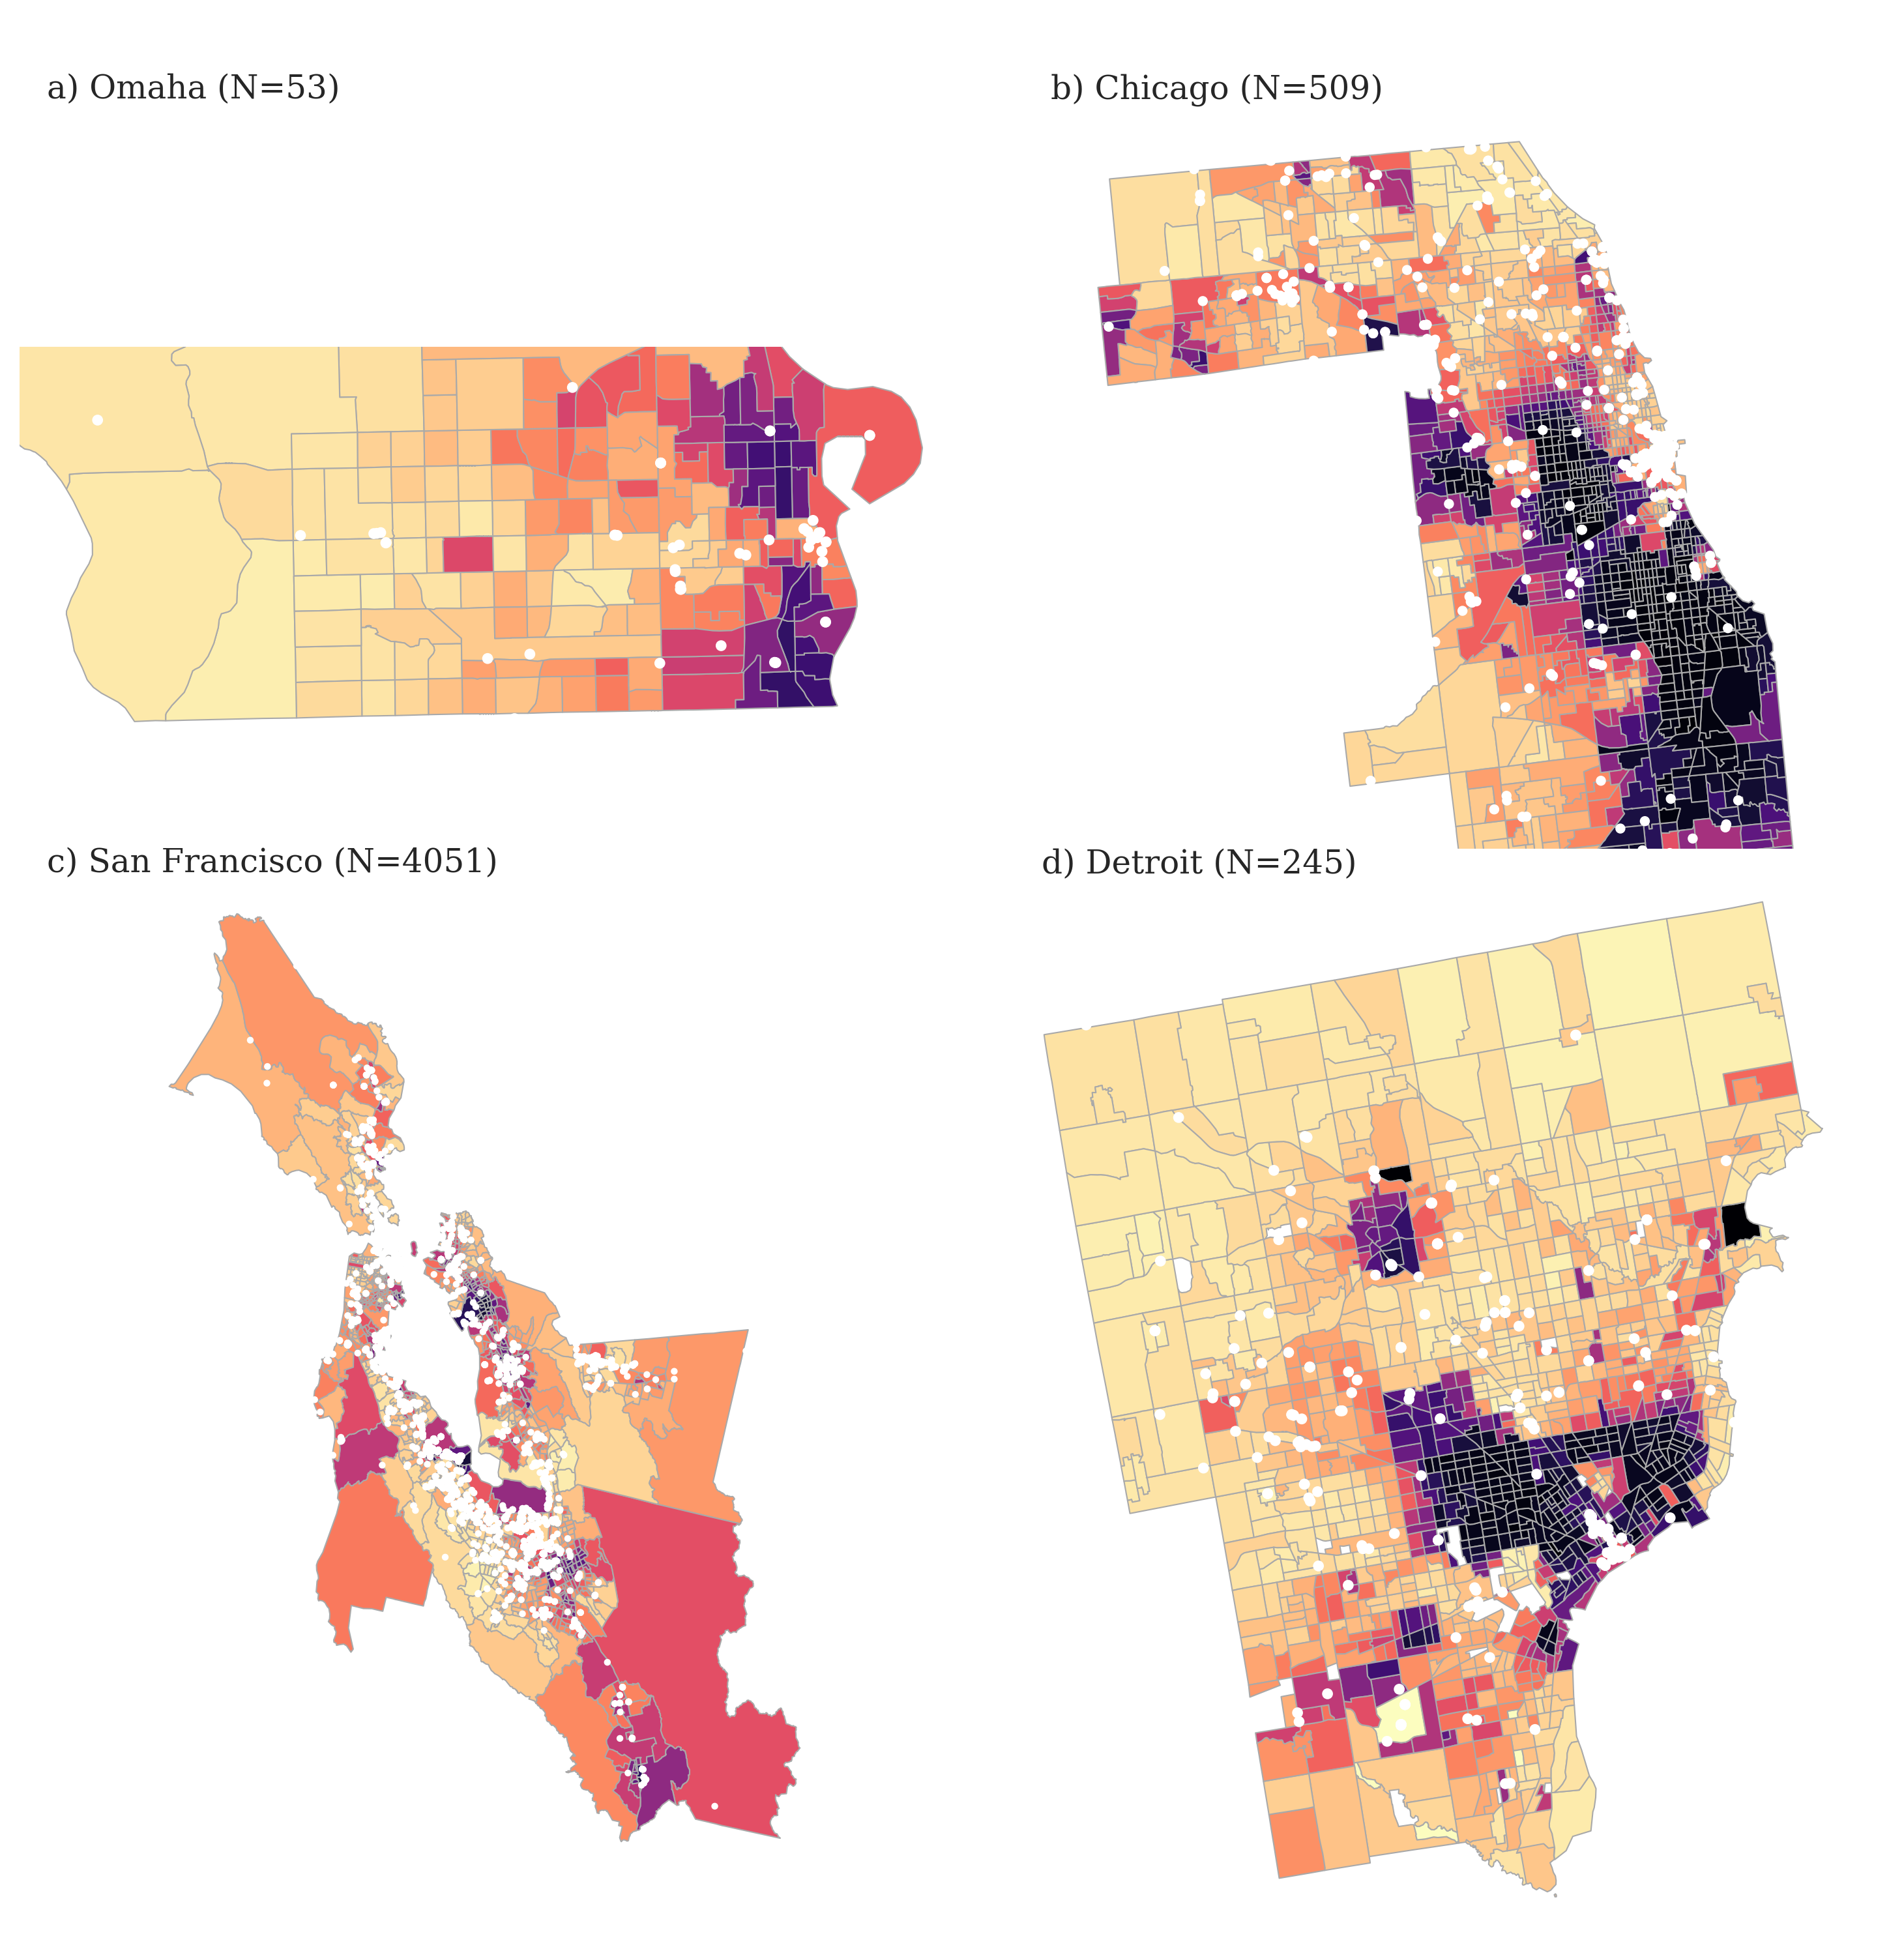
\includegraphics{TRB_2023_files/figure-pdf/fig-equity-output-1.png}

}

\caption{\label{fig-equity}Equity plot}

\end{figure}

Another simple descriptive comparison between the PEV and charging
station markets is shown in Figure 3. PEV sales market share is plotted
against charging stations per thousand residents as of 2020. While there
appears to be a positive correlation between these infrastructures,
there are clearly other factors at play - e.g., observe the difference
between California and Vermont.

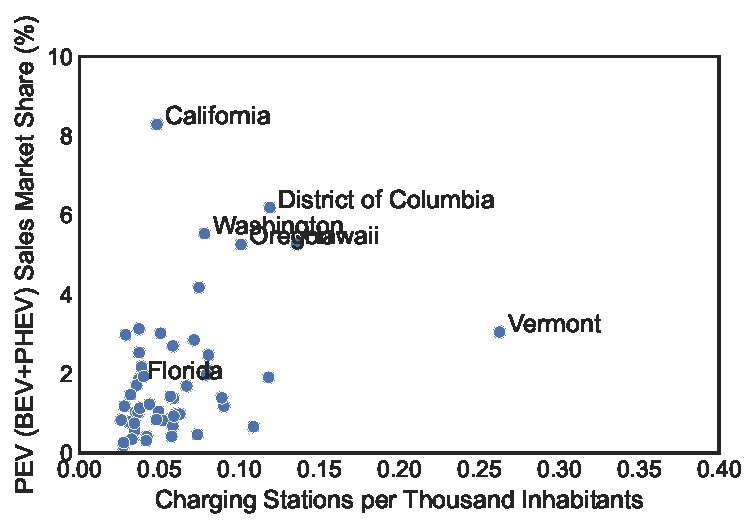
\includegraphics{TRB_2023_files/figure-pdf/cell-13-output-1.pdf}

\hypertarget{phasing-causality-analysis}{%
\subsection{Phasing Causality
Analysis}\label{phasing-causality-analysis}}

Before conducting the causality testing, we use Augmented Dickey-Fuller
(ADF) and Kwiatkouski-Phillips-Schmidt-Shin (KPSS) tests for
stationarity tests were applied to the aggregated US time series and its
first differenced analogue. In both cases, it was found that the time
series is non-stationary. ADF and KPSS tests were also iteratively
applied to each county time series with simiar results.

A limitation to the machine learning-based causality tests is that they
require large datasets to perform inference on a highly non-stationary
time series. Five annual datapoints is insufficient to run the tests. We
overcome this barrier by leveraging the spatio-temporal nature of our
dataset. The strategy is to consider each county as a slice of a
spatio-temporal series. We select only the 2020 data and assume that
charging stations and EV registrations in that year may be affected by
their corresponding observations in previous years but not observations
in other counties. This approach effectively defines a spatio-temporal
series with a maximum lag of four units (lagged 2018, 2016, 2014, and
2012) plus an instantaneous effect (2020). Figure Figure~\ref{fig-lags}
illustrates the concept for five random counties.

\begin{figure}

{\centering 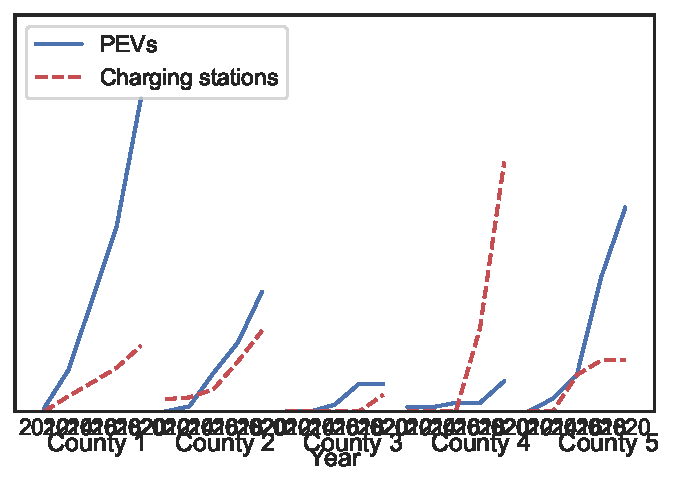
\includegraphics{TRB_2023_files/figure-pdf/fig-lags-output-1.pdf}

}

\caption{\label{fig-lags}Lags plot}

\end{figure}

We perform the non-linear causality tests using MLP, LSM, GRU, and ARIMA
models. Given that charging station data can be aggregated to annual
totals in every year, we also test both one and two year lags
alternatively considering charging stations and EV registrations as the
causal impetus. That is, we consider 2012, 2014, 2016, 2018, and 2020
station totals and 2011, 2015, 2017, and 2019 totals causing EV
registrations in the five available years, then add 2021 station totals
and consider EV registrations as causing charging station deployments.
In neither case are definitive results found to support either causal
mechanisms. These results indicate a feedback relationship between the
two variables of interest. While our spatio-temporal approach allows us
to perform these statistical tests, it does not allow us to test for
feedback effects because the underlying time series remains too short.

\begin{longtable}[]{@{}llllll@{}}
\toprule()
model & lag & cohens\_d\_pc & cohens\_d\_cp & cohens\_d\_pcl &
cohens\_d\_cpl \\
\midrule()
\endhead
ARIMA & 1 & 0.012 & 0.031 & 0.027 & 0.030 \\
ARIMA & 2 & 0.010 & 0.029 & 0.026 & 0.026 \\
ARIMA & 3 & 0.013 & 0.018 & 0.025 & 0.031 \\
ARIMA & 4 & 0.005 & 0.025 & 0.016 & 0.024 \\
ARIMA & 5 & 0.000 & 0.018 & 0.010 & 0.005 \\
GRU & 1 & 0.131 & 0.199 & 0.156 & 0.258 \\
LSTM & 1 & 0.240 & 0.231 & 0.133 & 0.035 \\
LSTM & 2 & 0.211 & 0.157 & 0.101 & 0.357 \\
LSTM & 3 & 0.196 & 0.069 & 0.145 & 0.062 \\
LSTM & 5 & 0.144 & 0.094 & 0.102 & 0.264 \\
MLP & 2 & 0.253 & 0.433 & 0.627 & 0.164 \\
MLP & 3 & 0.120 & 0.511 & 0.414 & 0.526 \\
MLP & 4 & 0.197 & 0.522 & 0.371 & 0.210 \\
MLP & 5 & 0.008 & 0.506 & 0.574 & 0.100 \\
NN & 1 & 0.160 & 0.007 & 0.003 & 0.136 \\
NN & 3 & 0.155 & 0.044 & 0.097 & 0.020 \\
NN & 4 & 0.053 & 0.064 & 0.036 & 0.049 \\
\bottomrule()
\end{longtable}

\hypertarget{dose-response-results}{%
\subsection{Dose-Response Results}\label{dose-response-results}}

With inclusive phasing causality results, we maintain the assumption
that charging stations cause EV registrations in the dose-response
analysis.

\begin{verbatim}
C:\Users\jhawkins17\Anaconda3\envs\geo_env\lib\site-packages\causal_curve\gps_core.py:452: UserWarning: KNOWN BUG: p-values computed in this summary are likely much smaller than they should be. 
 
Please do not make inferences based on these values! 

Collaborate on a solution, and stay up to date at: 
github.com/dswah/pyGAM/issues/163 

  self.gam_results.summary()
\end{verbatim}

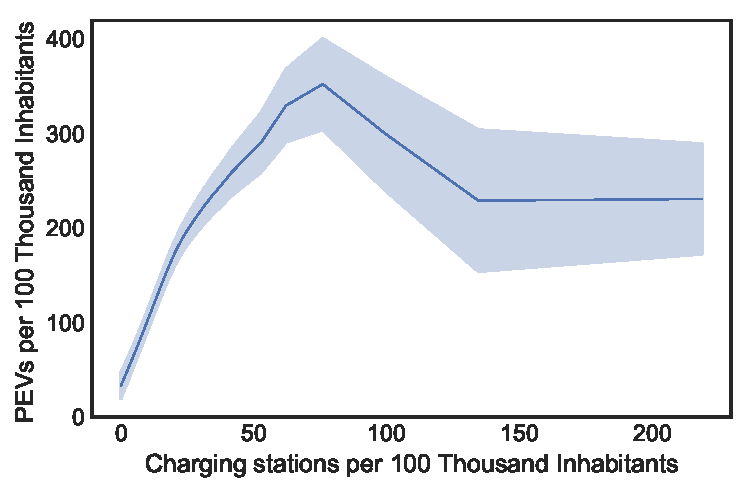
\includegraphics{TRB_2023_files/figure-pdf/cell-21-output-1.pdf}

\hypertarget{gps-model-results}{%
\subsection{GPS Model Results}\label{gps-model-results}}

\begin{longtable}[]{@{}lll@{}}
\toprule()
~ & est. & t-stat \\
\midrule()
\endhead
xW & 0.019 & 13.10 \\
Percent\_Minority & -7.3 & -1.28 \\
ABDPE001 & -0.28 & -4.75 \\
\bottomrule()
\end{longtable}

\hypertarget{mediation-effect-results}{%
\subsection{Mediation Effect Results}\label{mediation-effect-results}}

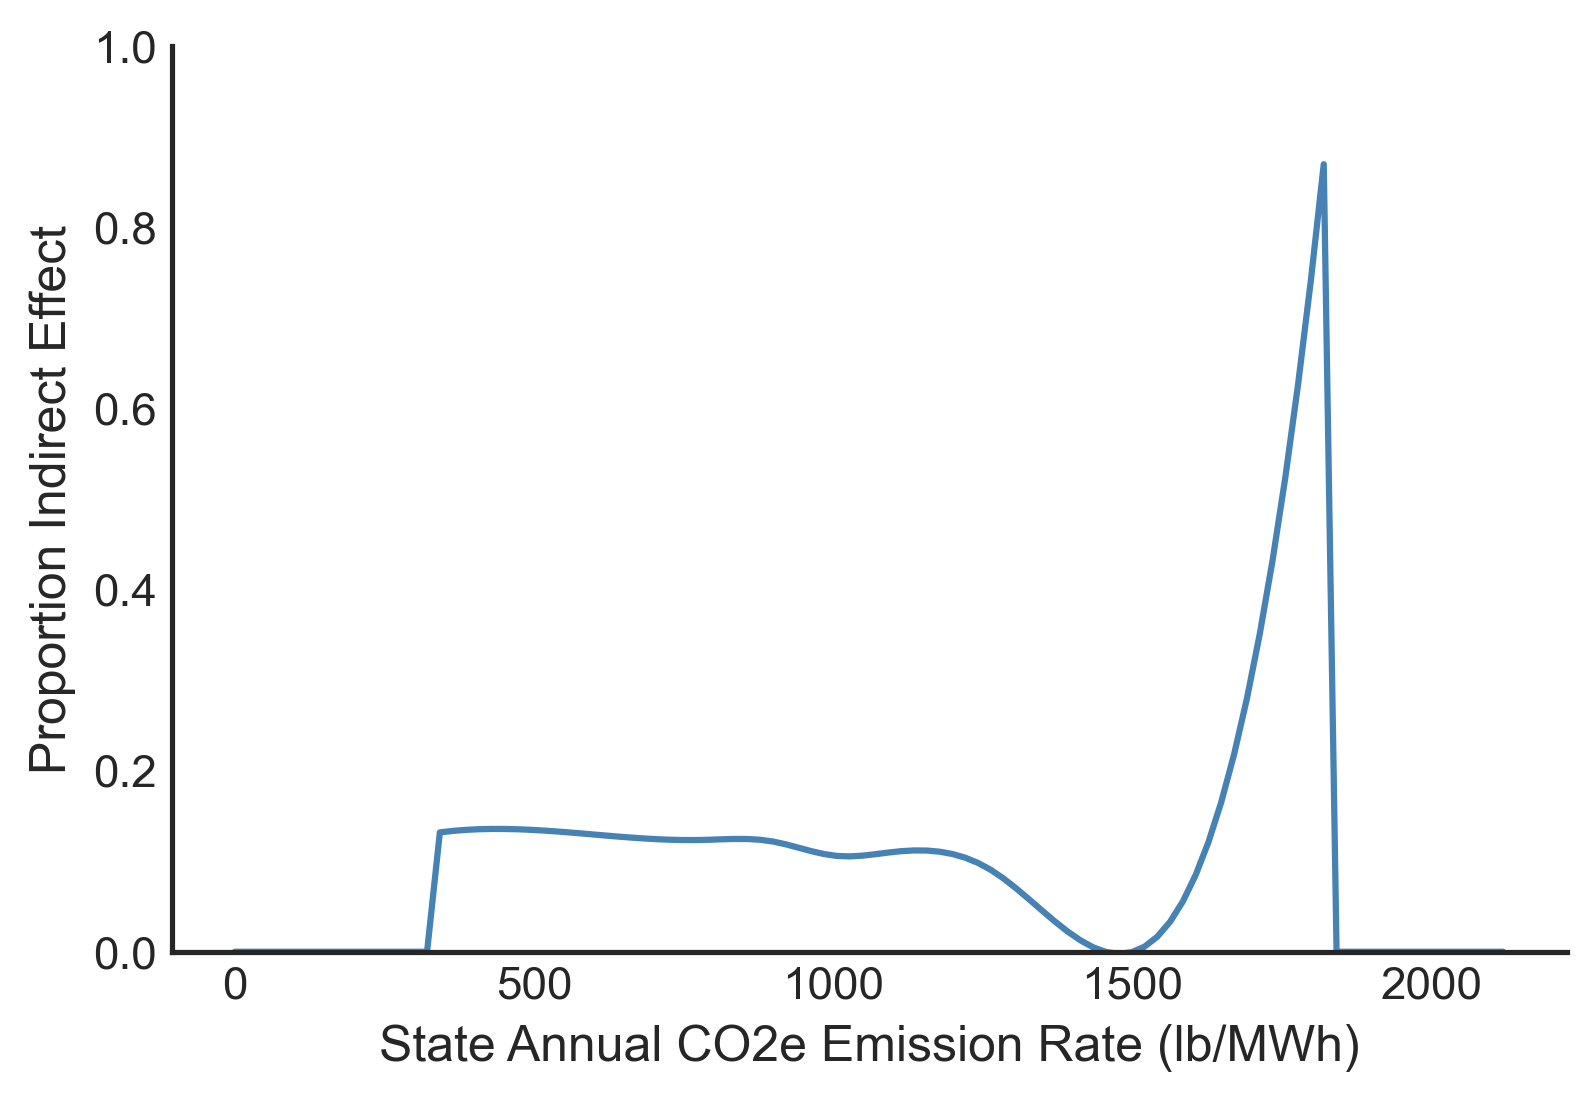
\includegraphics{TRB_2023_files/figure-pdf/cell-25-output-1.png}

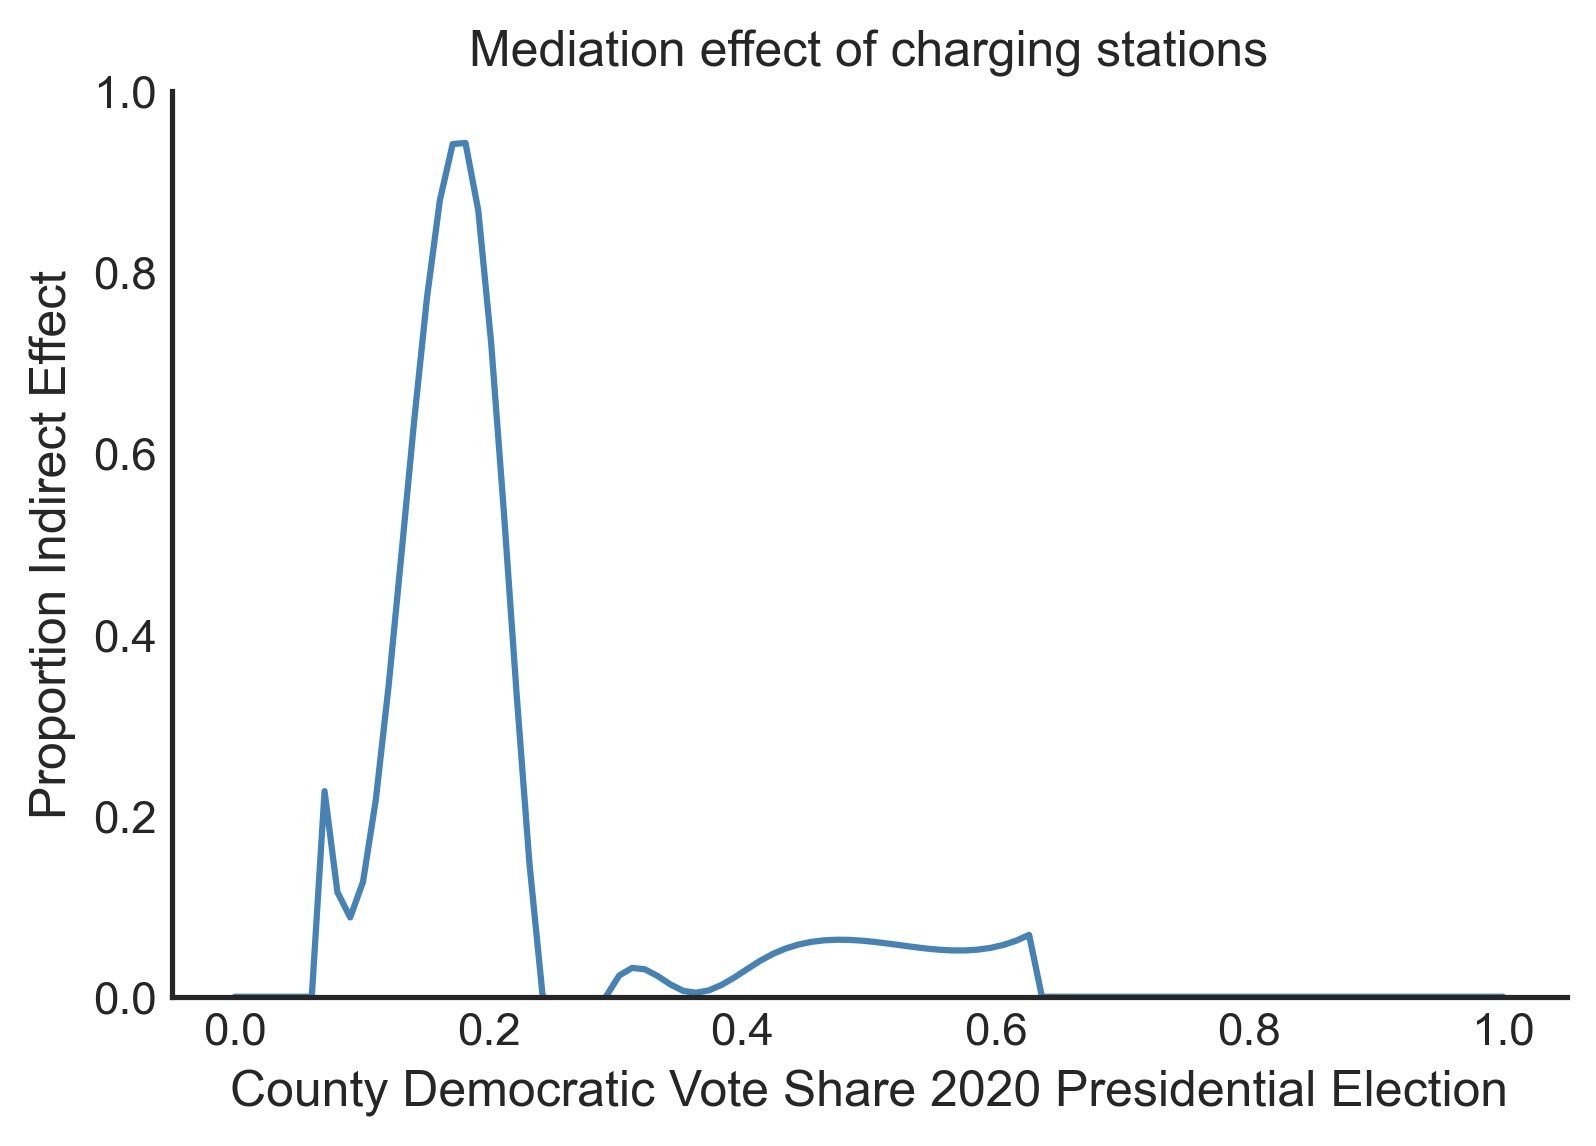
\includegraphics{TRB_2023_files/figure-pdf/cell-28-output-1.png}

\hypertarget{discussion-and-conclusions}{%
\section{Discussion and Conclusions}\label{discussion-and-conclusions}}

The results presented herein are preliminary and do not consider a key
dataset -- vehicle registrations. We will expand our analysis to a more
robust inferential study in the coming months. Our causal question is
what effect public charging stations have on electric vehicle
registrations at the county-level. The treatment variable is continuous
over the study period. We propose three causal identification
approaches. The first approach is a difference-in-differences approach
that is identified off state-level investments in charging stations by
year. The second approach is generalized propensity score matching using
federal election results, state-level greenhouse gas (GHG) emissions
factors, and demographic characteristics (e.g., racial composition,
median income, and population density) as inputs to the propensity
score.

The final causal inference approach, Granger causality, differs in that
it focuses on the temporal phasing of charging station installations and
PEV registration, whereas the other two approaches rely on Rubin's
potential outcome assumption (Reich et al. 2021). Granger causality
relies on the assumption that past treatment knowledge reduces
predictive uncertainty. It is a form of time series causal inference
that would fit the current context well.

\hypertarget{refs}{}
\begin{CSLReferences}{1}{0}
\leavevmode\vadjust pre{\hypertarget{ref-aultman-hall2018}{}}%
Aultman-Hall, Lisa. 2018. {``Incorporating Long-Distance Travel into
Transportation Planning in the United States.''}
\url{https://escholarship.org/uc/item/0ft8b3b5}.

\leavevmode\vadjust pre{\hypertarget{ref-elfalan2021}{}}%
Elfalan, Jonathan. 2021. {``Electric Car Range and Consumption.''}
\url{https://www.edmunds.com/car-news/electric-car-range-and-consumption-epa-vs-edmunds.html}.

\leavevmode\vadjust pre{\hypertarget{ref-melliger2018}{}}%
Melliger, Marc A., Oscar P. R. van Vliet, and Heikki Liimatainen. 2018.
{``Anxiety Vs Reality {\textendash} Sufficiency of Battery Electric
Vehicle Range in Switzerland and Finland.''} \emph{Transportation
Research Part D: Transport and Environment} 65 (December): 101--15.
\url{https://doi.org/10.1016/J.TRD.2018.08.011}.

\leavevmode\vadjust pre{\hypertarget{ref-musti2011}{}}%
Musti, Sashank, and Kara M. Kockelman. 2011. {``Evolution of the
Household Vehicle Fleet: Anticipating Fleet Composition, PHEV Adoption
and GHG Emissions in Austin, Texas.''} \emph{Transportation Research
Part A: Policy and Practice} 45 (8): 707--20.
\url{https://doi.org/10.1016/J.TRA.2011.04.011}.

\leavevmode\vadjust pre{\hypertarget{ref-reich2021}{}}%
Reich, Brian J., Shu Yang, Yawen Guan, Andrew B. Giffin, Matthew J.
Miller, and Ana Rappold. 2021. {``A Review of Spatial Causal Inference
Methods for Environmental and Epidemiological Applications.''}
\emph{International Statistical Review} 89 (3): 605--34.
\url{https://doi.org/10.1111/insr.12452}.

\leavevmode\vadjust pre{\hypertarget{ref-silvia2016}{}}%
Silvia, Chris, and Rachel M. Krause. 2016. {``Assessing the Impact of
Policy Interventions on the Adoption of Plug-in Electric Vehicles: An
Agent-Based Model.''} \emph{Energy Policy} 96 (September): 105--18.
\url{https://doi.org/10.1016/J.ENPOL.2016.05.039}.

\leavevmode\vadjust pre{\hypertarget{ref-sullivan2021}{}}%
Sullivan, Brian, and Harriet Taylor. 2021. {``The u.s. EV Charging
Network Isn't Ready for Your Family Road Trip, Let Alone the Expected
Wave of New Cars.''}
\url{https://www.cnbc.com/2021/08/24/cnbc-road-test-the-us-ev-charging-network-isnt-ready-for-your-family-road-trip-let-alone-the-expected-wave-of-new-cars.html}.

\leavevmode\vadjust pre{\hypertarget{ref-vehicletechnologyoffice2022}{}}%
Vehicle Technology Office. 2022. {``More Than Half of All Daily Trips
Were Less Than Three Miles in 2021.''}
\url{https://www.energy.gov/eere/vehicles/articles/fotw-1230-march-21-2022-more-half-all-daily-trips-were-less-three-miles-2021}.

\leavevmode\vadjust pre{\hypertarget{ref-wolbertus2018}{}}%
Wolbertus, Rick, Maarten Kroesen, Robert van den Hoed, and Caspar G.
Chorus. 2018. {``Policy Effects on Charging Behaviour of Electric
Vehicle Owners and on Purchase Intentions of Prospective Owners: Natural
and Stated Choice Experiments.''} \emph{Transportation Research Part D:
Transport and Environment} 62 (July): 283--97.
\url{https://doi.org/10.1016/j.trd.2018.03.012}.

\end{CSLReferences}



\end{document}
